\section{Ejercicios}
	
\begin{enumerate}
\item El interruptor de la Figura~\ref{fig.ej1_BT4} lleva cerrado un
  tiempo que se puede considerar infinito. En el instante $t=0$, se
  abre, permaneciendo en esta posición definitivamente. Calcular la
  expresión de la intensidad $i(t)$ desde $t=0$ en adelante.
  \begin{figure}[H]
    \centering 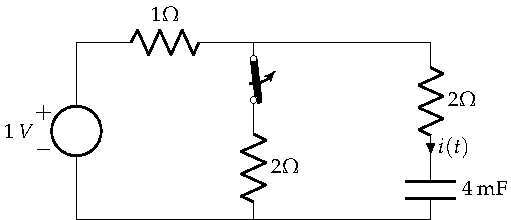
\includegraphics{../figs/ej1_BT4.pdf}
    \caption{Ejercicio 1}
    \label{fig.ej1_BT4}
  \end{figure}
  \emph{Sol.: $i(t)=\dfrac{1}{9}\; \mathrm{e}^{-\frac{t}{0.012}} A$}
\item El circuito de la Figura~\ref{fig.ej2_BT4} se encuentra en
  régimen permanente. En el instante $t=0$ se abre el
  interruptor. Calcular $u_1$ y $u_2$ para $t>0$.
  \begin{figure}[H]
    \centering 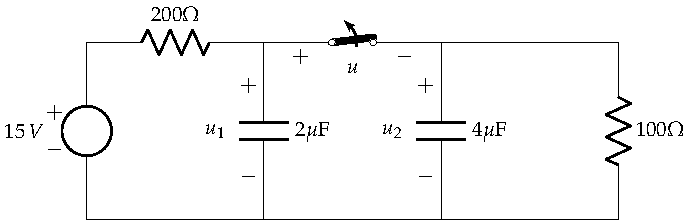
\includegraphics{../figs/ej2_BT4.pdf}
    \caption{Ejercicio 2}
    \label{fig.ej2_BT4}
  \end{figure}
  \emph{Sol.:
    $u_1(t)=15-10\,\mathrm{e}^{-2500\,t}\,V;\;
    u_2(t)=5\,\mathrm{e}^{-2500\,t}\,V$}
\item El interruptor del circuito de la Figura~\ref{fig.ej3_BT4} lleva
  cerrado un timepo que se considera infinito. En el instante $t=0$,
  se abre y permanece en dicha posición definitivamente. Hállese la
  expresión de $u(t)$ e $i(t)$ para $t>0$.
  \begin{figure}[H]
    \centering
    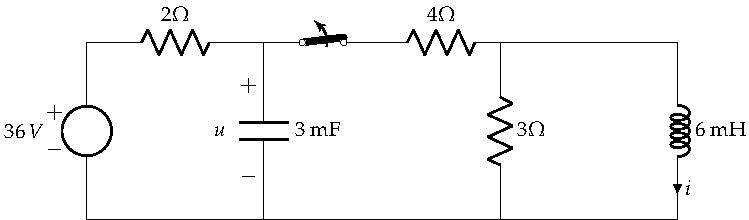
\includegraphics[width=0.65\linewidth]{../figs/ej3_BT4.pdf}
    \caption{Ejercicio 3}
    \label{fig.ej3_BT4}
  \end{figure}
  \emph{Sol.:
    $u(t)=36-12\,\mathrm{e}^{-166.67\,t}\,V;\;
    i(t)=6\,\mathrm{e}^{-500\,t}\,A$}
\item El circuito de la Figura~\ref{fig.ej4_BT4} lleva en esa posición
  un tiempo que se puede considerar infinito. En el instante $t=0$,
  ambos interruptores cambian su posición. Calcular la expresión de
  $u(t)$ para $t>0$.
  \begin{figure}[H]
    \centering
    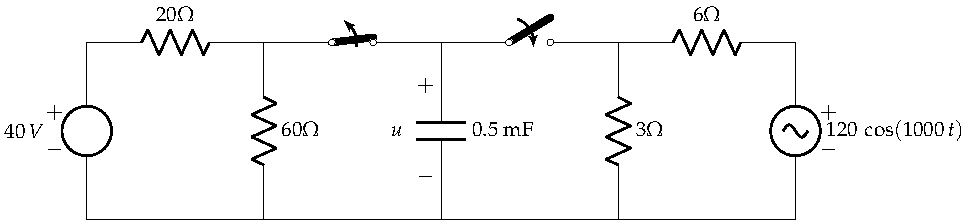
\includegraphics[width=.9\linewidth]{../figs/ej4_BT4.pdf}
    \caption{Ejercicio 4}
    \label{fig.ej4_BT4}
  \end{figure}
  \emph{Sol.:
    $u(t)=10\,\mathrm{e}^{-1000\,t}+20\sqrt{2}\,\cos\left(1000\,t-\frac{\pi}{4}\right)\,V$}
\item En el circuito de la Figura~\ref{fig.ej5_BT4}, se abre el
  interruptor después de un tiempo suficientemente grande para
  considerar que el circuito funcionaba en régimen
  permanente. Expresar las formas de onda de $i_1$, $i_2$ y $u_L$ para
  $t>0$, sabiendo que la fuente de tensión alterna es
  $e(t)=220\sqrt{2}\cos(100\pi\,t)$ V.
  \begin{figure}[H]
    \centering
    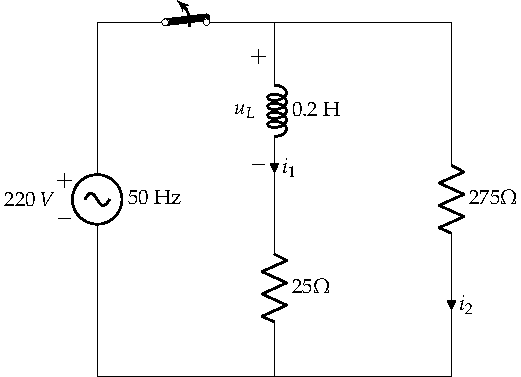
\includegraphics[width=0.45\linewidth]{../figs/ej5_BT4.pdf}
    \caption{Ejercicio 5}
    \label{fig.ej5_BT4}
  \end{figure}
  \emph{Sol.:
    $i_1(t)=1.7\,\mathrm{e}^{-1500\,t}\,A;\;i_2(t)=-1.7\,\mathrm{e}^{-1500\,t}\,A;\;
    u_L(t)=-510\,\mathrm{e}^{-1500\,t}\,V$}
\item En el circuito de la Figura~\ref{fig.ej6_BT4}, en $t = 0$ se
  cierra el interruptor. Obtener la expresión analítica de la
  intensidad $i(t)$, para $t > 0$.
  \begin{figure}[H]
    \centering 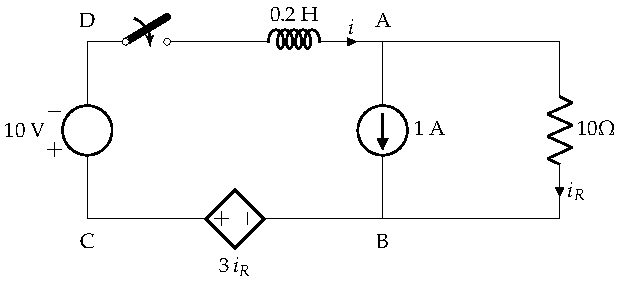
\includegraphics{../figs/ej6_BT4.pdf}
    \caption{Ejercicio 6}
    \label{fig.ej6_BT4}
  \end{figure}
  \emph{Sol.: $i(t)=\dfrac{3}{7}\,\mathrm{e}^{-35\,t}-\dfrac{3}{7}$}
\item En el circuito de la Figura~\ref{fig.ej7_BT4}, el interruptor
  permanece conectado en la posición mostrada el tiempo suficiente
  para que se encuentre en estado estacionario. En el instante $t=0$,
  cambia de posición. Obtener la expresión analítica de la tensión
  entre los bornes de la bobina.
  \begin{figure}[H]
    \centering 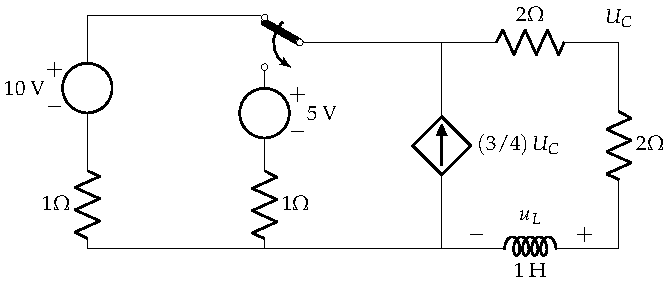
\includegraphics{../figs/ej7_BT4.pdf}
    \caption{Ejercicio 7}
    \label{fig.ej7_BT4}
  \end{figure}
  \emph{Sol.: $u(t)=-20\,\mathrm{e}^{-14\,t}\,V$}
\item En el circuito de la Figura~\ref{fig.FM_4_9}, calcular la tensión $u_C(t)$ para $t > 0$.\\
  Datos:
  $\epsilon_g = 4V;\; R_1 = {2}{\Omega};\; R_2 = {2}{\Omega};\; L =
  {1}{H};\; C = {0.25}{F} $
  \begin{figure}[H]
    \centering 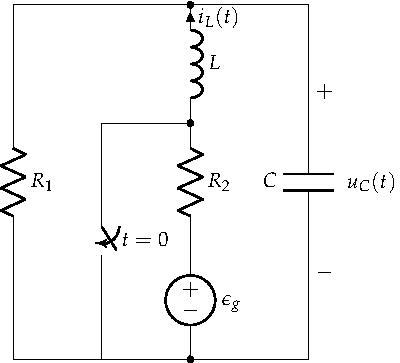
\includegraphics{../figs/FM_4_9.pdf}
    \caption{Ejercicio 8}
    \label{fig.FM_4_9}
  \end{figure}

  \emph{Sol.:
    $u_C(t)=
    \mathrm{e}^{-t}\left[2\,\cos(\sqrt{3}\,t)+\dfrac{2}{\sqrt{3}}\,\sin(\sqrt{3}\,t)\right]=\dfrac{4\sqrt{3}}{3}\,\mathrm{e}^{-t}\,\sin\left(\sqrt{3}\,t+\dfrac{\pi}{6}\right)$
    V}
  % \item El circuito de la Figura~\ref{fig.ej11_BT4} ha alcanzado el
  %   régimen permanente con el
  %   interruptor cerrado. El interruptor se abre en $t = 0$. Calcular las expresiones de la tensión en bornes del condensador y de la corriente por la bobina para $t > 0$.\\
  %   Datos:
  %
  %
  %
  %
  %
  %
  %
  %
  %
  %
  %
  %
  %
  %
  %
  %
  %
  %
  %
  %
  %
  %
  %
  %
  %
  %
  %
  %
  %
  %
  %
  %
  %
  %
  %
  %
  %
  %
  %
  %
  %
  %
  %
  %
  %
  %
  %
  %
  %
  %
  %
  %
  %
  %
  %
  %
  %
  %
  %
  %
  %
  %
  %
  %
  %
  %
  %
  %
  %
  %
  %
  %
  %
  %
  %
  %
  %
  %
  %
  %
  %
  %
  %
  %
  %
  %
  %
  %
  %
  %
  %
  %
  %
  %
  %
  %
  %
  %
  %
  %
  %
  %
  %
  %
  %
  %
  %
  %
  %
  %
  %
  %
  %
  %
  %
  %
  %
  %
  %
  %
  %
  %
  %
  %
  %
  %
  %
  %
  %
  %
  %
  %
  %
  %
  %
  %
  %
  %
  %
  %
  %
  %
  %
  %
  %
  %
  %
  %
  %
  %
  %
  %
  %
  %
  %
  %
  %
  %
  %
  %
  %
  %
  %
  %
  %
  %
  %
  %
  %
  %
  %
  %
  %
  %
  %
  %
  %
  %
  %
  %
  %
  %
  %
  %
  %
  %
  %
  %
  %
  %
  %
  %
  %
  %
  %
  %
  %
  %
  %
  %
  %
  %
  %
  %
  %
  %
  %
  %
  %
  %
  %
  %
  %
  %
  %
  %
  %
  %
  %
  %
  %
  %
  %
  %
  %
  %
  %
  %
  %
  %
  %
  %
  %
  %
  %
  %
  %
  %
  %
  %
  %
  %
  %
  %
  %
  %
  %
  %
  %
  %
  %
  %
  %
  %
  %
  %
  %
  %
  %
  %
  %
  %
  %
  %
  %
  %
  %
  %
  %
  %
  %
  %
  %
  %
  %
  %
  %
  %
  %
  %
  %
  %
  %
  %
  %
  %
  %
  %
  %
  %
  %
  %
  %
  %
  %
  %
  %
  %
  %
  %
  %
  %
  %
  %
  %
  %
  %
  %
  %
  %
  %
  %
  %
  %
  %
  %
  %
  %
  %
  %
  %
  %
  %
  %
  %
  %
  %
  %
  %
  %
  %
  %
  %
  %
  %
  %
  %
  %
  %
  %
  %
  %
  %
  %
  %
  %
  %
  %
  %
  %
  %
  %
  %
  %
  %
  %
  %
  %
  %
  %
  %
  %
  %
  %
  %
  %
  %
  %
  %
  %
  %
  %
  %
  %
  %
  %
  %
  %
  %
  %
  %
  %
  %
  %
  %
  %
  %
  %
  %
  %
  %
  %
  %
  %
  %
  %
  %
  %
  %
  %
  %
  %
  %
  %
  %
  %
  %
  %
  %
  %
  %
  %
  %
  %
  %
  %
  %
  %
  %
  %
  %
  %
  %
  %
  %
  %
  %
  %
  %
  %
  %
  %
  %
  %
  %
  %
  %
  %
  %
  %
  %
  %
  %
  %
  %
  %
  %
  %
  %
  %
  %
  %
  %
  %
  %
  %
  %
  %
  %
  %
  %
  %
  %
  %
  %
  %
  %
  %
  %
  %
  %
  %
  %
  %
  %
  %
  %
  %
  %
  %
  %
  %
  %
  %
  %
  %
  %
  %
  %
  %
  %
  %
  %
  %
  %
  %
  %
  %
  %
  %
  %
  %
  %
  %
  %
  %
  %
  %
  %
  %
  %
  %
  %
  %
  %
  %
  %
  %
  %
  %
  %
  %
  %
  %
  %
  %
  %
  %
  %
  %
  %
  %
  %
  %
  %
  %
  %
  %
  %
  %
  %
  %
  %
  %
  %
  %
  %
  %
  %
  %
  %
  %
  %
  %
  %
  %
  %
  %
  %
  %
  %
  %
  %
  %
  %
  %
  %
  %
  %
  %
  %
  %
  %
  %
  %
  %
  %
  %
  %
  %
  %
  %
  %
  %
  %
  %
  %
  %
  %
  %
  %
  %
  %
  %
  %
  %
  %
  %
  %
  %
  %
  %
  %
  %
  %
  %
  %
  %
  %
  %
  %
  %
  %
  %
  %
  %
  %
  %
  %
  %
  %
  %
  %
  %
  %
  %
  %
  %
  %
  %
  %
  %
  %
  %
  %
  %
  %
  %
  %
  %
  %
  %
  %
  %
  %
  %
  %
  %
  %
  %
  %
  %
  %
  %
  %
  %
  %
  %
  %
  %
  %
  %
  %
  %
  %
  %
  %
  %
  %
  %
  %
  %
  %
  %
  %
  %
  %
  %
  %
  %
  %
  %
  %
  %
  %
  %
  %
  %
  %
  %
  %
  %
  %
  %
  %
  %
  %
  %
  %
  %
  %
  %
  %
  %
  %
  %
  %
  %
  %
  %
  %
  %
  %
  %
  %
  %
  %
  %
  %
  %
  %
  %
  %
  %
  %
  %
  %
  %
  %
  %
  %
  %
  %
  %
  %
  %
  %
  %
  %
  %
  %
  %
  %
  %
  %
  %
  %
  %
  %
  %
  %
  %
  %
  %
  %
  %
  %
  %
  %
  %
  %
  %
  %
  %
  %
  %
  %
  %
  %
  %
  %
  %
  %
  %
  %
  %
  %
  %
  %
  %
  %
  %
  %
  %
  %
  %
  %
  %
  %
  %
  %
  %
  %
  %
  %
  %
  %
  %
  %
  %
  %
  %
  %
  %
  %
  %
  %
  %
  %
  %
  %
  %
  %
  %
  %
  %
  %
  %
  %
  %
  %
  %
  %
  %
  %
  %
  %
  %
  %
  %
  %
  %
  %
  %
  %
  %
  %
  %
  %
  %
  %
  %
  %
  %
  %
  %
  %
  %
  %
  %
  %
  %
  %
  %
  %
  %
  %
  %
  %
  %
  %
  %
  %
  %
  %
  %
  %
  %
  %
  %
  %
  %
  %
  %
  %
  %
  %
  %
  %
  %
  %
  %
  %
  %
  %
  %
  %
  %
  %
  %
  %
  %
  %
  %
  %
  %
  %
  %
  %
  %
  %
  %
  %
  %
  %
  %
  %
  %
  %
  %
  %
  %
  %
  %
  %
  %
  %
  %
  %
  %
  %
  %
  %
  %
  %
  %
  %
  %
  %
  %
  %
  %
  %
  %
  %
  %
  %
  %
  %
  %
  %
  %
  %
  %
  %
  %
  %
  %
  %
  %
  %
  %
  %
  %
  %
  %
  %
  %
  %
  %
  %
  %
  %
  %
  %
  %
  %
  %
  %
  %
  %
  %
  %
  %
  %
  %
  %
  %
  %
  %
  %
  %
  %
  %
  %
  %
  %
  %
  %
  %
  %
  %
  %
  %
  %
  %
  %
  %
  %
  %
  %
  %
  %
  %
  %
  %
  %
  %
  %
  %
  %
  %
  %
  %
  %
  %
  %
  %
  %
  %
  %
  %
  %
  %
  %
  %
  %
  %
  %
  %
  %
  %
  %
  %
  %
  %
  %
  %
  %
  %
  %
  %
  %
  %
  %
  %
  %
  %
  %
  %
  %
  %
  %
  %
  %
  %
  %
  %
  %
  %
  %
  %
  %
  %
  %
  %
  %
  %
  %
  %
  %
  %
  %
  %
  %
  %
  %
  %
  %
  %
  %
  %
  %
  %
  %
  %
  %
  %
  %
  %
  %
  %
  %
  %
  %
  %
  %
  %
  %
  %
  %
  %
  %
  %
  %
  %
  %
  %
  %
  %
  %
  %
  %
  %
  %
  %
  %
  %
  %
  %
  %
  %
  %
  %
  %
  %
  %
  %
  %
  %
  %
  %
  %
  %
  %
  %
  %
  %
  %
  %
  %
  %
  %
  %
  %
  %
  %
  %
  %
  %
  %
  %
  %
  %
  %
  %
  %
  %
  %
  %
  %
  %
  %
  %
  %
  %
  %
  %
  %
  %
  %
  %
  %
  %
  %
  %
  %
  %
  %
  %
  %
  %
  %
  %
  %
  %
  %
  %
  %
  %
  %
  %
  %
  %
  %
  %
  %
  %
  %
  %
  %
  %
  %
  %
  %
  %
  %
  %
  %
  %
  %
  %
  %
  %
  %
  %
  %
  %
  %
  %
  %
  %
  %
  %
  %
  %
  %
  %
  %
  %
  %
  %
  %
  %
  %
  %
  %
  %
  %
  %
  %
  %
  %
  %
  %
  %
  %
  %
  %
  %
  %
  %
  %
  %
  %
  %
  %
  %
  %
  %
  %
  %
  %
  %
  %
  %
  %
  %
  %
  %
  %
  %
  %
  %
  %
  %
  %
  %
  %
  %
  %
  %
  %
  %
  %
  %
  %
  %
  %
  %
  %
  %
  %
  %
  %
  %
  %
  %
  %
  %
  %
  %
  %
  %
  %
  %
  %
  %
  %
  %
  %
  %
  %
  %
  %
  %
  %
  %
  %
  %
  %
  %
  %
  %
  %
  %
  %
  %
  %
  %
  %
  %
  %
  %
  %
  %
  %
  %
  %
  %
  %
  %
  %
  %
  %
  %
  %
  %
  %
  %
  %
  %
  %
  %
  %
  %
  %
  %
  %
  %
  %
  %
  %
  %
  %
  %
  %
  %
  %
  %
  %
  %
  %
  %
  %
  %
  %
  %
  %
  %
  %
  %
  %
  %
  %
  %
  %
  %
  %
  %
  %
  %
  %
  %
  %
  %
  %
  %
  %
  %
  %
  %
  %
  %
  %
  %
  %
  %
  %
  %
  %
  %
  %
  %
  %
  %
  %
  %
  %
  %
  %
  %
  %
  %
  %
  %
  %
  %
  %
  %
  %
  %
  %
  %
  %
  %
  %
  %
  %
  %
  %
  %
  %
  %
  %
  %
  %
  %
  %
  %
  %
  %
  %
  %
  %
  %
  %
  %
  %
  %
  %
  %
  %
  %
  %
  %
  %
  %
  %
  %
  %
  %
  %
  %
  %
  %
  %
  %
  %
  %
  %
  %
  %
  %
  %
  %
  %
  %
  %
  %
  %
  %
  %
  %
  %
  %
  %
  %
  %
  %
  %
  %
  %
  %
  %
  %
  %
  %
  %
  %
  %
  %
  %
  %
  %
  %
  %
  %
  %
  %
  %
  %
  %
  %
  %
  %
  %
  %
  %
  %
  %
  %
  %
  %
  %
  %
  %
  %
  %
  %
  %
  %
  %
  %
  %
  %
  %
  %
  %
  %
  %
  %
  %
  %
  %
  %
  %
  %
  %
  %
  %
  %
  %
  %
  %
  %
  %
  %
  %
  %
  %
  %
  %
  %
  %
  %
  %
  %
  %
  %
  %
  %
  %
  %
  %
  %
  %
  %
  %
  %
  %
  %
  %
  %
  %
  %
  %
  %
  %
  %
  %
  %
  %
  %
  %
  %
  %
  %
  %
  %
  %
  %
  %
  %
  %
  %
  %
  %
  %
  %
  %
  %
  %
  %
  %
  %
  %
  %
  %
  %
  %
  %
  %
  %
  %
  %
  %
  %
  %
  %
  %
  %
  %
  %
  %
  %
  %
  %
  %
  %
  %
  %
  %
  %
  %
  %
  %
  %
  %
  %
  %
  %
  %
  %
  %
  %
  %
  %
  %
  %
  %
  %
  %
  %
  %
  %
  %
  %
  %
  %
  %
  %
  %
  %
  %
  %
  %
  %
  %
  %
  %
  %
  %
  %
  %
  %
  %
  %
  %
  %
  %
  %
  %
  %
  %
  %
  %
  %
  %
  %
  %
  %
  %
  %
  %
  %
  %
  %
  %
  %
  %
  %
  %
  %
  %
  %
  %
  %
  %
  %
  %
  %
  %
  %
  %
  %
  %
  %
  %
  %
  %
  %
  %
  %
  %
  %
  %
  %
  %
  %
  %
  %
  %
  %
  %
  %
  %
  %
  %
  %
  %
  %
  %
  %
  %
  %
  %
  %
  %
  %
  %
  %
  %
  %
  %
  %
  %
  %
  %
  %
  %
  %
  %
  %
  %
  %
  %
  %
  %
  %
  %
  %
  %
  %
  %
  %
  %
  %
  %
  %
  %
  %
  %
  %
  %
  %
  %
  %
  %
  %
  %
  %
  %
  %
  %
  %
  %
  %
  %
  %
  %
  %
  %
  %
  %
  %
  %
  %
  %
  %
  %
  %
  %
  %
  %
  %
  %
  %
  %
  %
  %
  %
  %
  %
  %
  %
  %
  %
  %
  %
  %
  %
  %
  %
  %
  %
  %
  %
  %
  %
  %
  %
  %
  %
  %
  %
  %
  %
  %
  %
  %
  %
  %
  %
  %
  %
  %
  %
  %
  %
  %
  %
  %
  %
  %
  %
  %
  %
  %
  %
  %
  %
  %
  %
  %
  %
  %
  %
  %
  %
  %
  %
  %
  %
  %
  %
  %
  %
  %
  %
  %
  %
  %
  %
  %
  %
  %
  %
  %
  %
  %
  %
  %
  %
  %
  %
  %
  %
  %
  %
  %
  %
  %
  %
  %
  %
  %
  %
  %
  %
  %
  %
  %
  %
  %
  %
  %
  %
  %
  %
  %
  %
  %
  %
  %
  %
  %
  %
  %
  %
  %
  %
  %
  %
  %
  %
  %
  %
  %
  %
  %
  %
  %
  %
  %
  %
  %
  %
  %
  %
  %
  %
  %
  %
  %
  %
  %
  %
  %
  %
  %
  %
  %
  %
  %
  %
  %
  %
  %
  %
  %
  %
  %
  %
  %
  %
  %
  %
  %
  %
  %
  %
  %
  %
  %
  %
  %
  %
  %
  %
  %
  %
  %
  %
  %
  %
  %
  %
  %
  %
  %
  %
  %
  %
  %
  %
  %
  %
  %
  %
  %
  %
  %
  %
  %
  %
  %
  %
  %
  %
  %
  %
  %
  %
  %
  %
  %
  %
  %
  %
  %
  %
  %
  %
  %
  %
  %
  %
  %
  %
  %
  %
  %
  %
  %
  %
  %
  %
  %
  %
  %
  %
  %
  %
  %
  %
  %
  %
  %
  %
  %
  %
  %
  %
  %
  %
  %
  %
  %
  %
  %
  %
  %
  %
  %
  %
  %
  %
  %
  %
  %
  %
  %
  %
  %
  %
  %
  %
  %
  %
  %
  %
  %
  %
  %
  %
  %
  %
  %
  %
  %
  %
  %
  %
  %
  %
  %
  %
  %
  %
  %
  %
  %
  %
  %
  %
  %
  %
  %
  %
  %
  %
  %
  %
  %
  %
  %
  %
  %
  %
  %
  %
  %
  %
  %
  %
  %
  %
  %
  %
  %
  %
  %
  %
  %
  %
  %
  %
  %
  %
  %
  %
  %
  %
  %
  %
  %
  %
  %
  %
  %
  %
  %
  %
  %
  %
  %
  %
  %
  %
  %
  %
  %
  %
  %
  %
  %
  %
  %
  %
  %
  %
  %
  %
  %
  %
  %
  %
  %
  %
  %
  %
  %
  %
  %
  %
  %
  %
  %
  %
  %
  %
  %
  %
  %
  %
  %
  %
  %
  %
  %
  %
  %
  %
  %
  %
  %
  %
  %
  %
  %
  %
  %
  %
  %
  %
  %
  %
  %
  %
  %
  %
  %
  %
  %
  %
  %
  %
  %
  %
  %
  %
  %
  %
  %
  %
  %
  %
  %
  %
  %
  %
  %
  %
  %
  %
  %
  %
  %
  %
  %
  %
  %
  %
  %
  %
  %
  %
  %
  %
  %
  %
  %
  %
  %
  %
  %
  %
  %
  %
  %
  %
  %
  %
  %
  %
  %
  %
  %
  %
  %
  %
  %
  %
  %
  %
  %
  %
  %
  %
  %
  %
  %
  %
  %
  %
  %
  %
  %
  %
  %
  %
  %
  %
  %
  %
  %
  %
  %
  %
  %
  %
  %
  %
  %
  %
  %
  %
  %
  %
  %
  %
  %
  %
  %
  %
  %
  %
  %
  %
  %
  %
  %
  %
  %
  %
  %
  %
  %
  %
  %
  %
  %
  %
  %
  %
  %
  %
  %
  %
  %
  %
  %
  %
  %
  %
  %
  %
  %
  %
  %
  %
  %
  %
  %
  %
  %
  %
  %
  %
  %
  %
  %
  %
  %
  %
  %
  %
  %
  %
  %
  %
  %
  %
  %
  %
  %
  %
  %
  %
  %
  %
  %
  %
  %
  %
  %
  %
  %
  %
  %
  %
  %
  %
  %
  %
  %
  %
  %
  %
  %
  %
  %
  %
  %
  %
  %
  %
  %
  %
  %
  %
  %
  %
  %
  %
  %
  %
  %
  %
  %
  %
  %
  %
  %
  %
  %
  %
  %
  %
  %
  %
  %
  %
  %
  %
  %
  %
  %
  %
  %
  %
  %
  %
  %
  %
  %
  %
  %
  %
  %
  %
  %
  %
  %
  %
  %
  %
  %
  %
  %
  %
  %
  %
  %
  %
  %
  %
  %
  %
  %
  %
  %
  %
  %
  %
  %
  %
  %
  %
  %
  %
  %
  %
  %
  %
  %
  %
  %
  %
  %
  %
  %
  %
  %
  %
  %
  %
  %
  %
  %
  %
  %
  %
  %
  %
  %
  %
  %
  %
  %
  %
  %
  %
  %
  %
  %
  %
  %
  %
  %
  %
  %
  %
  %
  %
  %
  %
  %
  %
  %
  %
  %
  %
  %
  %
  %
  %
  %
  %
  %
  %
  %
  %
  %
  %
  %
  %
  %
  %
  %
  %
  %
  %
  %
  %
  %
  %
  %
  %
  %
  %
  %
  %
  %
  %
  %
  %
  %
  %
  %
  %
  %
  %
  %
  %
  %
  %
  %
  %
  %
  %
  %
  %
  %
  %
  %
  %
  %
  %
  %
  %
  %
  %
  %
  %
  %
  %
  %
  %
  %
  %
  %
  %
  %
  %
  %
  %
  %
  %
  %
  %
  %
  %
  %
  %
  %
  %
  %
  %
  %
  %
  %
  %
  %
  %
  %
  %
  %
  %
  %
  %
  %
  %
  %
  %
  %
  %
  %
  %
  %
  %
  %
  %
  %
  %
  %
  %
  %
  %
  %
  %
  %
  %
  %
  %
  %
  %
  %
  %
  %
  %
  %
  %
  %
  %
  %
  %
  %
  %
  %
  %
  %
  %
  %
  %
  %
  %
  %
  %
  %
  %
  %
  %
  %
  %
  %
  %
  %
  %
  %
  %
  %
  %
  %
  %
  %
  %
  %
  %
  %
  %
  %
  %
  %
  %
  %
  %
  %
  %
  %
  %
  %
  %
  %
  %
  %
  %
  %
  %
  %
  %
  %
  %
  %
  %
  %
  %
  %
  %
  %
  %
  %
  %
  %
  %
  %
  %
  %
  %
  %
  %
  %
  %
  %
  %
  %
  %
  %
  %
  %
  %
  %
  %
  %
  %
  %
  %
  %
  %
  %
  %
  %
  %
  %
  %
  %
  %
  %
  %
  %
  %
  %
  %
  %
  %
  %
  %
  %
  %
  %
  %
  %
  %
  %
  %
  %
  %
  %
  %
  %
  %
  %
  %
  %
  %
  %
  %
  %
  %
  %
  %
  %
  %
  %
  %
  %
  %
  %
  %
  %
  %
  %
  %
  %
  %
  %
  %
  %
  %
  %
  %
  %
  %
  %
  %
  %
  %
  %
  %
  %
  %
  %
  %
  %
  %
  %
  %
  %
  %
  %
  %
  %
  %
  %
  %
  %
  %
  %
  %
  %
  %
  %
  %
  %
  %
  %
  %
  %
  %
  %
  %
  %
  %
  %
  %
  %
  %
  %
  %
  %
  %
  %
  %
  %
  %
  %
  %
  %
  %
  %
  %
  %
  %
  %
  %
  %
  %
  %
  %
  %
  %
  %
  %
  %
  %
  %
  %
  %
  %
  %
  %
  %
  %
  %
  %
  %
  %
  %
  %
  %
  %
  %
  %
  %
  %
  %
  %
  %
  %
  %
  %
  %
  %
  %
  %
  %
  %
  %
  %
  %
  %
  %
  %
  %
  %
  %
  %
  %
  %
  %
  %
  %
  %
  %
  %
  %
  %
  %
  %
  %
  %
  %
  %
  %
  %
  %
  %
  %
  %
  %
  %
  %
  %
  %
  %
  %
  %
  %
  %
  %
  %
  %
  %
  %
  %
  %
  %
  %
  %
  %
  %
  %
  %
  %
  %
  %
  %
  %
  %
  %
  %
  %
  %
  %
  %
  %
  %
  %
  %
  %
  %
  %
  %
  %
  %
  %
  %
  %
  %
  %
  %
  %
  %
  %
  %
  %
  %
  %
  %
  %
  %
  %
  %
  %
  %
  %
  %
  %
  %
  %
  %
  %
  %
  %
  %
  %
  %
  %
  %
  %
  %
  %
  %
  %
  %
  %
  %
  %
  %
  %
  %
  %
  %
  %
  %
  %
  %
  %
  %
  %
  %
  %
  %
  %
  %
  %
  %
  %
  %
  %
  %
  %
  %
  %
  %
  %
  %
  %
  %
  %
  %
  %
  %
  %
  %
  %
  %
  %
  %
  %
  %
  %
  %
  %
  %
  %
  %
  %
  %
  %
  %
  %
  %
  %
  %
  %
  %
  %
  %
  %
  %
  %
  %
  %
  %
  %
  %
  %
  %
  %
  %
  %
  %
  %
  %
  %
  %
  %
  %
  %
  %
  %
  %
  %
  %
  %
  %
  %
  %
  %
  %
  %
  %
  %
  %
  %
  %
  %
  %
  %
  %
  %
  %
  %
  %
  %
  %
  %
  %
  %
  %
  %
  %
  %
  %
  %
  %
  %
  %
  %
  %
  %
  %
  %
  %
  %
  %
  %
  %
  %
  %
  %
  %
  %
  %
  %
  %
  %
  %
  %
  %
  %
  %
  %
  %
  %
  %
  %
  %
  %
  %
  %
  %
  %
  %
  %
  %
  %
  %
  %
  %
  %
  %
  %
  %
  %
  %
  %
  %
  %
  %
  %
  %
  %
  %
  %
  %
  %
  %
  %
  %
  %
  %
  %
  %
  %
  %
  %
  %
  %
  %
  %
  %
  %
  %
  %
  %
  %
  %
  %
  %
  %
  %
  %
  %
  %
  %
  %
  %
  %
  %
  %
  %
  %
  %
  %
  %
  %
  %
  %
  %
  %
  %
  %
  %
  %
  %
  %
  %
  %
  %
  %
  %
  %
  %
  %
  %
  %
  %
  %
  %
  %
  %
  %
  %
  %
  %
  %
  %
  %
  %
  %
  %
  %
  %
  %
  %
  %
  %   $\epsilon_g = {10}{V};\; R_1 = {10}{\Omega};\; R_2 = {5}{\Omega};\;L = {2.5}{H};\; C = {0.2}{F}$
% \begin{figure}[H]
%     \centering
%     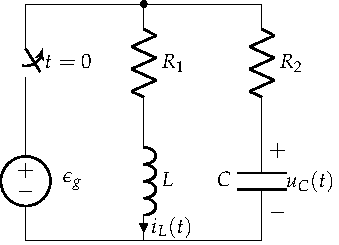
\includegraphics{../figs/FM_4_8.pdf}
%     \caption{Ejercicio 11}
%     \label{fig.ej11_BT4}
% \end{figure}

% \emph{Sol.: $i_L(t)=0.651\,\mathrm{e}^{0.317\,t}+0.349\,\mathrm{e}^{-6.317\,t};\; u_C(t)=10.281\,\mathrm{e}^{0.317\,t}-0.277\,\mathrm{e}^{-6.317\,t}$ A}
\item En el circuito de la Figura~\ref{fig.ej12_BT4} el interruptor ha estado cerrado durante un tiempo elevado y, en $t = 0$, se abre. Determinar la expresión de la corriente $i_L(t)$ para $t>0$, especificando el tipo de transitorio.\\
Datos: $E_g = 500 V;\; R_1 = 375 \Omega;\; R_2 = 125\Omega;\; L_1 = 40 mH;\; L_2 = 40 mH;\; C = 1 \mu F$
\begin{figure}[H]
    \centering
    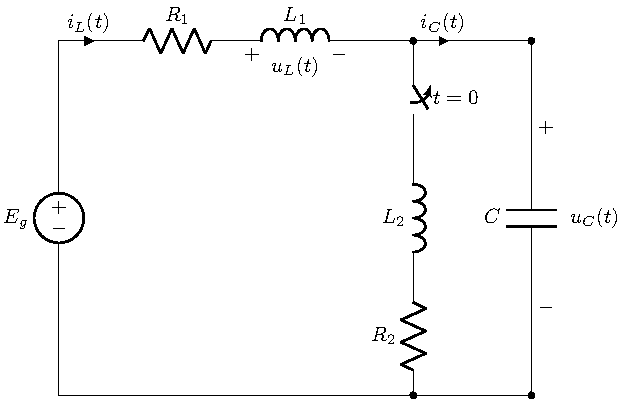
\includegraphics{../figs/ej12_BT4.pdf}
    \caption{Ejercicio 9}
    \label{fig.ej12_BT4}
\end{figure}

	   \emph{Sol.: $i_L(t)= \mathrm{e}^{-4687.5\,t}\left[\cos(1739.93\,t)+2.69\,\sin(1739.93\,t)\right]=2.87\,\mathrm{e}^{-t}\,\sin\left(1739.93\,t+1.215\right)$ A}
	    
\item En el circuito de la Figura~\ref{fig.ej11_BT4}, determinar la tensión $u$ en el condensador a partir del instante en que se abre el interruptor, el cual lleva cerrado desde un tiempo infinito.
\begin{figure}[H]
    \centering
    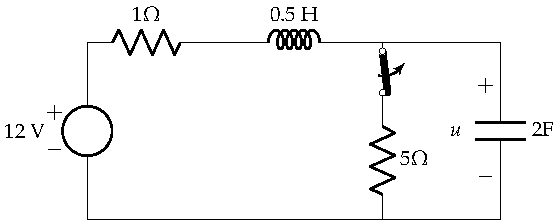
\includegraphics{../figs/ej11_BT4.pdf}
    \caption{Ejercicio 10}
    \label{fig.ej11_BT4}
\end{figure}	 
\emph{Sol.: $u(t)=12-\mathrm{e}^{-t}\left(2+2\,t\right)$ V}

	    
	   % \item El circuito de la Figura~\ref{fig.ej10_BT4} se encuentra en régimen permanente, con el condensador descargado. En un instante dado, que se toma como origen de tiempos, se cierra el interruptor. Determinar $u(t)$ para $t>0$. 
	   % \begin{figure}[H]
	   %     \centering
	   %     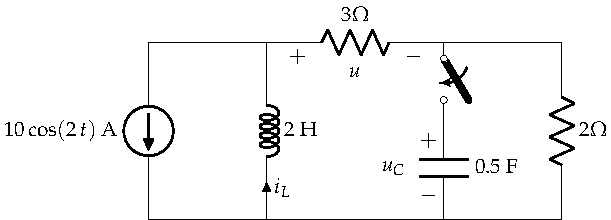
\includegraphics{../figs/ej10_BT4.pdf}
	   %     \caption{Ejercicio 10}
	   %     \label{fig.ej10_BT4}
	   % \end{figure}
	    
	\end{enumerate}
 
%%% Local Variables:
%%% mode: latex
%%% TeX-master: "enunciados_ejercicios_TC"
%%% ispell-local-dictionary: "castellano"
%%% End:
